\subsubsection{Set 3 - Greenyard Maaseik}
\label{sec:PL1_Greenyard3}
Voor de opslagen en receptie wordt figuur \ref{fig:PL1ServeMaaseik3} bekeken. 
Het aantal opslagen is bij beide hetzelfde getal. Ook het aantal perfecte (0) opslagen zijn gelijk. De AI-invoer is echter veel minder kritisch dan de manuele invoer. De manuele invoer heeft meer opslagen met score 3, terwijl de AI-invoer meer opslagen heeft met score 1 en 2.

Heel opvallend hier is dat er 8 recepties met score 0 (slechte receptie) zijn bij de manuele invoer en maar 1 bij de AI-invoer. Score 1 werd aan 8 recepties gegeven door de manuele invoer en 10 door de AI. Vijf recepties kregen score 2 door de scouter en zeven recepties kregen diezelfde score door de AI.

\begin{figure}[ht]
\centering
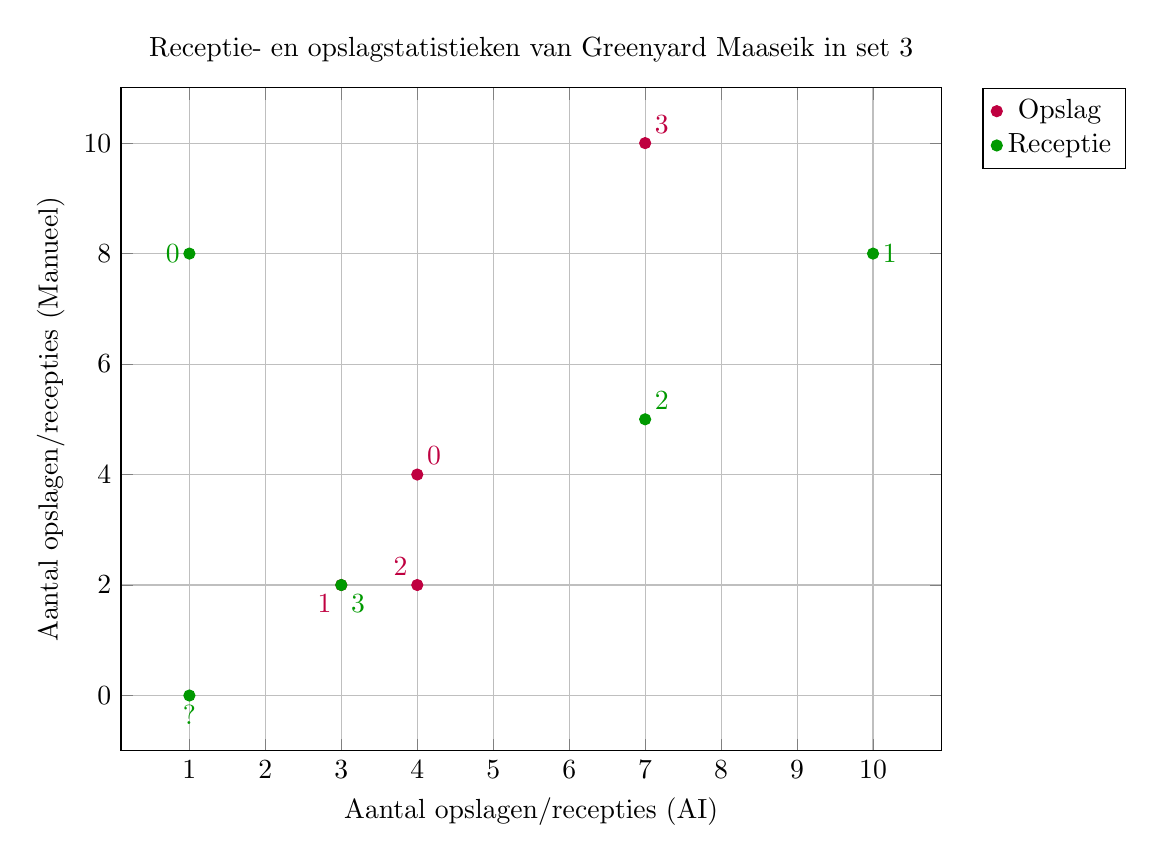
\begin{tikzpicture}
  \begin{axis}[
    title={Receptie- en opslagstatistieken van Greenyard Maaseik in set 3},
    xlabel={Aantal opslagen/recepties (AI)},
    ylabel={Aantal opslagen/recepties (Manueel)},
    grid=major,
    legend style={at={(1.05,1)}, anchor=north west},
    width=12cm,
    height=10cm,
    enlargelimits=0.1,
  ]

  % Opslag (paars)
  \addplot[
    only marks,
    mark=*,
    color=purple,
  ] table {
    x y
    4 4
    3 2
    4 2
    7 10
  };
  \addlegendentry{Opslag}

  % Labels opslag
  \node at (axis cs:4,4) [anchor=south west, purple] {0};
  \node at (axis cs:3,2) [anchor=north east, purple] {1};
  \node at (axis cs:4,2) [anchor=south east, purple] {2};
  \node at (axis cs:7,10) [anchor=south west, purple] {3};

  % Receptie (groen)
  \addplot[
    only marks,
    mark=*,
    color=green!60!black,
  ] table {
    x y
    3 2
    7 5
    10 8
    1 8
    1 0
  };
  \addlegendentry{Receptie}

  % Labels receptie
  \node at (axis cs:3,2) [anchor=north west, green!60!black] {3};
  \node at (axis cs:7,5) [anchor=south west, green!60!black] {2};
  \node at (axis cs:10,8) [anchor=west, green!60!black] {1};
  \node at (axis cs:1,8) [anchor=east, green!60!black] {0};
  \node at (axis cs:1,0) [anchor=north, green!60!black] {?};

  \end{axis}
\end{tikzpicture}
\caption{AI invoer versus manuele invoer, ingedeeld in opslag en receptie, voor Greenyard Maaseik in set 3.}
\label{fig:PL1ServeMaaseik3}
\end{figure}

In tabellen \ref{tab:PL1SetMaaseikMan3} en \ref{tab:PL1SetDigMaaseikAI3} wordt de spelverdeling weergegeven. De hoeveelheden zijn hier zeer verschillend. Bij sommige spelers geeft de manuele invoer ze meer, bij andere dan weer meer door de AI. Volgens manuele invoer heeft Jolan Cox ook vijf keer aan spelverdeling gedaan, terwijl dit door AI geen enkele keer was. Dawid Pawlun heeft door de AI 17 keer aan spelverdeling gedaan, terwijl dit manueel maar 14 keer was. Dit is een verschil van 3. Dit is een groot verschil, maar het kan zijn dat de AI deze als spelverdeling heeft gezien, terwijl dit manueel niet zo was.

Ook bij de verdeding, tabel \ref{tab:PL1DigMaaseikMan3} en \ref{tab:PL1SetDigMaaseikAI3}, zijn er duidelijke verschillen te zien. Hier zijn er ook meerdere spelers die verschillende hoeveelheden verdedigingsacties hebben gekregen. Dit kan iets te maken hebben dat de verdediging buiten het beeld van de camera is gebeurd, waardoor de AI dit niet heeft kunnen registreren.

\begin{table}[ht!]
    \centering
    \scriptsize
    \begin{tabular}{|l|c|c|c|c|c|c|c|c|c|} \hline
        \textbf{Speler} & *E\% & Tot & = & / & - & ! & + & \# \\ \hline
        Samuel Fafchamps  & 100\% & 1 &  &  &  &  & 1 &  \\ 
        Renet Vancker & 100\% & 3 &  &  &  &  & 3 &  \\
        Jolan Cox & 100\% & 5 &  &  &  &  & 5 &  \\ 
        Landon Douglas Currie & 100\% & 1 &  &  &  &  & 1 &  \\ 
        Dawid Pawlun & 100\% & 14 &  &  &  &  & 11 & 3 \\ 
        Hampus Ekstrand & 100\% & 1 &  &  &  &  & 1 &  \\
        Pierre Perin & 100\% & 4 &  &  &  &  & 4 &  \\ \hline
    \end{tabular}
    \caption[Manueel ingevoerde spelverdelingsstatistieken voor Greenyard Maaseik in set 3]{\label{tab:PL1SetMaaseikMan3}Manueel ingevoerde spelverdeling statistieken voor Greenyard Maaseik in set 3.}
\end{table}

\begin{table}[ht!]
    \centering
    \scriptsize
    \begin{tabular}{|l|c|c|c|c|c|c|c|c|c|} \hline
        \textbf{Speler} & *E\% & Tot & = & / & - & ! & + & \#\\ \hline
        Renet Vancker & 0\% & 2 & 1 &  & 1 &  &  &  \\ 
        Jolan Cox & 75\% & 4 &  & 1 & 1 &  & 2 &  \\ 
        Landon Douglas Currie & 50\% & 2 &  &  & 1 &  & 1 &  \\ 
        Dawid Pawlun & 33\% & 3 &  &  & 2 &  & 1 &  \\ 
        Miquel Angel Fornés & 0\% & 2 & 1 &  & 1 &  &  &  \\ 
        Pierre Perin & 67\% & 3 &  &  & 1 &  & 2 &  \\ \hline
    \end{tabular}
    \caption[Manueel ingevoerde verdedigingsstatistieken voor Greenyard Maaseik in set 3]{\label{tab:PL1DigMaaseikMan3}Manueel ingevoerde verdediging statistieken voor Greenyard Maaseik in set 3.}
\end{table}

\begin{table}[ht!]
  \centering
  \scriptsize
  \begin{tabular}{|l|c|c|c|c|c|c|c|} \hline
    \textbf{Speler} & Ast & TA & SE & PCT & DS & DE \\ \hline
    Samuel Fafchamps &  & 1 &  & 0\% &  &  \\
    Renet Vancker &  & 3 &  & 0\% & 1 &  \\
    Jolan Cox &  &  &  &  &  5 &  \\
    Landon Douglas Currie &  & 2 &  & 0\% & 3 & 1 \\
    Dawid Pawlun & 6 & 17 &  & 35\% & 4 &  \\
    Tijmen Bus &  & 1 &  & 0\% & 1 &  \\
    Hampus Ekstrand & 1 & 2 & & 50\% &  &  \\
    Piere Perin &  & 5 &  & 0\% & 2 &  \\  \hline
  \end{tabular}
  \caption[Spelverdelings- en verdedigingsstatistieken gemaakt door Balltime AI voor Greenyard Maaseik in set 3]{\label{tab:PL1SetDigMaaseikAI3}Spelverdelings- en verdedigingsstatistieken gemaakt door Balltime AI voor Greenyard Maaseik in set 3.}
\end{table}

Tabel \ref{tab:PL1AttMaaseikMan3}, \ref{tab:PL1BlockMaaseikMan3} en \ref{tab:PL1AttBlockMaaseikAI3} tonen de de aanval en blokstatistieken gemaakt door de AI en de manuele invoer voor Greenyard Maaseik in set 3. 

De aanvallen worden correct geregisteerd door de AI, behalve bij één speler. Jolan Cox heeft een aanval te minder dan bij de manuele invoer. 

De aanvallen en blokkeringen worden door de AI niet beoordeeld op kwaliteit. Ook worden de blokkeringen op een totaal andere manier bekeken door de AI. Dit systeem geeft geen duidelijke blokpunten. Dit is echter wel van belang.

\begin{table}[ht!]
    \centering
    \scriptsize
    \begin{tabular}{|l|c|c|c|c|c|c|c|c|c|} \hline
        \textbf{Speler} & *E\% & Tot & = & / & - & ! & + & \#\\ \hline
        Andris Sirjakovs & -67\% & 3 &  & 2 &  &  & 1 &  \\ 
        Jolan Cox & 0\% & 5 &  & 1 & 3 &  &  & 1 \\ 
        Dawid Pawlun & 0\% & 2 & 1 &  &  &  &  & 1 \\ 
        Tijmen Bus & -25\% & 4 & 1 & 1 &  & 1 &  & 1 \\ 
        Miquel Angel Fornés & 50\% & 2 &  &  &  &  & 1 & 1 \\ 
        Hampus Ekstrand & 12\% & 8 & 1 & 1 & 1 & 1 & 1 & 3 \\ 
        Pierre Perin  & 17\% & 6 & 1 &  & 2 & 1 &  & 2 \\ \hline
    \end{tabular}
   \caption[Manueel ingevoerde aanvalsstatistieken voor Greenyard Maaseik in set 3]{\label{tab:PL1AttMaaseikMan3}Manueel ingevoerde aanvalsstatistieken voor Greenyard Maaseik in set 3.}
\end{table}

\begin{table}[ht!]
    \centering
    \scriptsize
    \begin{tabular}{|l|c|c|c|c|c|c|c|c|c|} \hline
        \textbf{Speler} & *E\% & Tot & = & / & - & ! & + & \#\\ \hline
        Samuel Fafchamps & 50\% & 2 &  &  &  & 1 &  & 1 \\ 
        Jolan Cox & -100\% & 1 & 1 &  &  &  &  &  \\
        Dawid Pawlun & -25\% & 4 & 1 & 1 &  &  & 1 & 1 \\
        Miquel Angel Fornés & 0\% & 3 & 1 &  &  & 1 &  & 1 \\ 
        Pierre Perin & 0\% & 1 &  &  &  & 1 &  &  \\ \hline
    \end{tabular}
    \caption[Manueel ingevoerde blokstatistieken voor Greenyard Maaseik in set 3]{\label{tab:PL1BlockMaaseikMan3}Manueel ingevoerde blokstatistieken voor Greenyard Maaseik in set 3.}
\end{table}

\begin{table}[ht!]
  \centering
  \scriptsize
  \begin{tabular}{|l|c|c|c|c|c|c|c|c|c|c|c|} \hline
    \textbf{Speler} &  K & E & TA & Atk\% & Kill\% & Error\% & BS & BA & BE \\ \hline
    Samuel Fafchamps &   &   &   &   &   &   & 1 &  & \\
    Andris Sirjakovs &  & 2 & 3 & -0.67 & 0\% & 67\% &   &  & \\
    Jolan Cox & 1 & 1 & 6 & 0.00 & 17\% & 17\% &  &  & \\
    Dawid Pawlun & 1 & 1 & 2 & 0.00 & 50\% & 50\% & 1 &  & \\
    Tijmen Bus &  & 2 & 4 & -0.50 & 0\% & 50\% & &  &  \\
    Miquel Angel Fornés & 1 &  & 2 & 0.50 & 50\% & 0\% & 1 & & \\
    Hampus Ekstrand & 3 & 1 & 8 & 0.25 & 38\% & 12\% &   &   &  \\
    Piere Perin & 2 & 1 & 6 & 0.17 & 33\% & 17 \%&  &  & \\ \hline
  \end{tabular}
  \caption[Aanvals- en blokstatistieken gemaakt door Balltime AI voor Greenyard Maaseik in set 3]{\label{tab:PL1AttBlockMaaseikAI3}Aanvals- en blokstatistieken gemaakt door Balltime AI voor Greenyard Maaseik in set 3.}
\end{table}
